% Koko
\documentclass[blue,normal,cn]{elegantnote}
\usepackage{array}
\usepackage{courier}
\usepackage{xcolor}
\usepackage{zhnumber}
\usepackage{ulem}
\usepackage{float}

\definecolor{ans}{RGB}{230, 74, 25}

\definecolor{light-gray}{gray}{0.95}
\newcommand{\code}[1]{\colorbox{light-gray}{\texttt{#1}}}
\newfontfamily\courier{Courier New}
\lstset{linewidth=1.1\textwidth,
	numbers=left,
	basicstyle=\small\courier,
	numberstyle=\tiny\courier,
	keywordstyle=\color{blue}\courier,
	commentstyle=\it\color[cmyk]{1,0,1,0}\courier, 
	stringstyle=\it\color[RGB]{128,0,0}\courier,
	frame=single,
	backgroundcolor=\color[RGB]{245,245,244},
	breaklines,
	extendedchars=false, 
	xleftmargin=2em,xrightmargin=2em, aboveskip=1em,
	tabsize=4, 
	showspaces=false
	basicstyle=\small\courier
}
\title{实验 2: 流水线及流水线中的冲突}
\version{$\aleph$}
\date{\zhtoday}

\begin{document}
\author{
  \begin{tabular}[t]{cccc}
    于海鑫     & 田静悦     & 赵泉斌     & 黄震\footnote{以学号顺序排序} \\
    2017211240 & 2017211259 & 2017211268 & 2017211274
  \end{tabular}
}
\maketitle

\section{实验目的}
\begin{enumerate}
  \item 加深对计算机流水线基本概念的理解
  \item 理解 MIPS 结构如何用 5 段流水线来实现,理解各段的功能和基本操作
  \item 加深对数据冲突和资源冲突的理解,理解这两类冲突对 CPU 性能的影响
  \item 进一步理解解决数据冲突的方法,掌握如何应用定向技术来减少数据冲突引起的停顿
\end{enumerate}

\section{实验平台}

实验平台采用指令级和流水线操作级模拟器 \code{MIPSsim}。

\section{实验内容和步骤}

首先要阅读 MIPSsim 模拟器的使用方法(见附录),然后了解 MIPSsim 的指令系统和汇编语言。

\begin{enumerate}[wide=0pt, listparindent=2em, parsep=0pt]
  \item 启动 MIPSsim
  \item 进一步理解流水线窗口中各段的功能,掌握各流水寄存器的含义。(鼠标双击各段,即可看到各流水寄存器的内容)
  \item 载入一个样例程序(在本模拟器所在文件夹下的“样例程序”文件夹中),然后分别以单步执行一个周期、执行多个周期、连续执行、设置断点等方式运行程序,观察程序的执行情况,观察 CPU 中寄存器和存储器内容的变化,特别是流水寄存器内容的变化。
  \item 选择配置菜单中的“流水方式”选项,使模拟器工作于流水方式下
  \item 观察程序在流水方式下的执行情况。
  \item 观察和分析结构冲突对 CPU 性能的影响,步骤如下

        \begin{itemize}[leftmargin=3em, listparindent=2em, parsep=0pt]
          \item 加载 \code{structure\_hz.s}(在模拟器所在文件夹下的“样例程序”文件夹中)。
          \item 执行该程序,找出存在结构冲突的指令对以及导致结构冲突的部件。


                \textcolor{ans}{\code{0x20} 前的任意一条指令都会引发结构冲突,冲突部件为浮点数加法器(fadd)。}


          \item 记录由结构冲突引起的停顿周期数,计算停顿周期数占总执行周期数的百分比。


                \textcolor{ans} {停顿周期:41}

                \textcolor{ans} {占比:78.84615\%}

                \textcolor{ans}{运行报告:}
                \begin{lstlisting}
汇总:
    执行周期总数:52
    ID段执行了10条指令

  硬件配置:
    内存容量:4096 B
    加法器个数:1		执行时间(周期数):6
    乘法器个数:1		执行时间(周期数)7		
    除法器个数:1		执行时间(周期数)10		
    定向机制:不采用

  停顿(周期数):
    RAW停顿:0		占周期总数的百分比:0%
    其中:
      load停顿:0		占所有RAW停顿的百分比:0%
      浮点停顿:0		占所有RAW停顿的百分比:0%
    WAW停顿:0		占周期总数的百分比:0%
    结构停顿:35		占周期总数的百分比:67.30769%
    控制停顿:0		占周期总数的百分比:0%
    自陷停顿:6		占周期总数的百分比:11.53846%
    停顿周期总数:41	占周期总数的百分比:78.84615%

  分支指令:
    指令条数:0		占指令总数的百分比:0%
    其中:
      分支成功:0		占分支指令数的百分比:0%
      分支失败:0		占分支指令数的百分比:0%

  load/store指令:
    指令条数:0		占指令总数的百分比:0%
    其中:
      load:0		占load/store指令数的百分比:0%
      store:0		占load/store指令数的百分比:0%

  浮点指令:
    指令条数:8		占指令总数的百分比:80%
    其中:
      加法:8		占浮点指令数的百分比:100%
      乘法:0		占浮点指令数的百分比:0%
      除法:0		占浮点指令数的百分比:0%

  自陷指令:
    指令条数:1		占指令总数的百分比:10%
\end{lstlisting}

          \item 把浮点加法器的个数改为 4 个。
          \item 再重复 1-3 的步骤。

                \textcolor{ans} {停顿周期:8}

                \textcolor{ans} {占比:42.10526\%}

                \textcolor{ans}{运行报告:}
                \begin{lstlisting}
  汇总:
    执行周期总数:19
    ID段执行了10条指令

  硬件配置:
    内存容量:4096 B
    加法器个数:4		执行时间(周期数):6
    乘法器个数:1		执行时间(周期数)7		
    除法器个数:1		执行时间(周期数)10		
    定向机制:不采用

  停顿(周期数):
    RAW停顿:0		占周期总数的百分比:0%
    其中:
      load停顿:0		占所有RAW停顿的百分比:0%
      浮点停顿:0		占所有RAW停顿的百分比:0%
    WAW停顿:0		占周期总数的百分比:0%
    结构停顿:2		占周期总数的百分比:10.52632%
    控制停顿:0		占周期总数的百分比:0%
    自陷停顿:6		占周期总数的百分比:31.57895%
    停顿周期总数:8	占周期总数的百分比:42.10526%

  分支指令:
    指令条数:0		占指令总数的百分比:0%
    其中:
      分支成功:0		占分支指令数的百分比:0%
      分支失败:0		占分支指令数的百分比:0%

  load/store指令:
    指令条数:0		占指令总数的百分比:0%
    其中:
      load:0		占load/store指令数的百分比:0%
      store:0		占load/store指令数的百分比:0%

  浮点指令:
    指令条数:8		占指令总数的百分比:80%
    其中:
      加法:8		占浮点指令数的百分比:100%
      乘法:0		占浮点指令数的百分比:0%
      除法:0		占浮点指令数的百分比:0%

  自陷指令:
    指令条数:1		占指令总数的百分比:10%
\end{lstlisting}
          \item 分析结构冲突对 CPU 性能的影响,讨论解决结构冲突的方法。

                \textcolor{ans}{影响:当发生冲突时,流水线会出现停顿从而降低CPU的性能}

                \textcolor{ans}{解决方式:增加部件,设置独立寄存器}
        \end{itemize}

  \item 观察数据冲突并用定向技术来减少停顿,步骤如下:
        \begin{itemize}[leftmargin=3em, listparindent=2em, parsep=0pt]
          \item 全部复位。
          \item 加载 \code{data\_hz.s}(在模拟器所在文件夹下的“样例程序”文件夹中)。
          \item 关闭定向功能(在“配置”菜单下选择取消“定向”)。
          \item 用单步执行一个周期的方式执行该程序,观察时钟周期图,列出什么时刻发生了 RAW 冲突。

                \textcolor{ans}{第 4, 6, 7, 9, 10, 13, 14, 17, 18, 20, 21, 25, 26, 28, 29, 32, 33, 36, 37, 39, 40, 44, 45, 47, 48, 51, 52, 55, 56, 58 周期发生了 RAW 冲突。}

          \item 记录数据冲突引起的停顿周期数以及程序执行的总时钟周期数,计算停顿时钟周期数占总执行周期数的百分比。

                \textcolor{ans} {停顿周期:31}

                \textcolor{ans} {总周期:65}

                \textcolor{ans} {占比:47.69231\%}

                \textcolor{ans}{运行报告:}
                \begin{lstlisting}
  汇总:
    执行周期总数:65
    ID段执行了29条指令

  硬件配置:
    内存容量:4096 B
    加法器个数:1		执行时间(周期数):6
    乘法器个数:1		执行时间(周期数)7		
    除法器个数:1		执行时间(周期数)10		
    定向机制:不采用

  停顿(周期数):
    RAW停顿:31		占周期总数的百分比:47.69231%
    其中:
      load停顿:12		占所有RAW停顿的百分比:38.70968%
      浮点停顿:0		占所有RAW停顿的百分比:0%
    WAW停顿:0		占周期总数的百分比:0%
    结构停顿:0		占周期总数的百分比:0%
    控制停顿:3		占周期总数的百分比:4.615385%
    自陷停顿:1		占周期总数的百分比:1.538462%
    停顿周期总数:35	占周期总数的百分比:53.84615%

  分支指令:
    指令条数:3		占指令总数的百分比:10.34483%
    其中:
      分支成功:2		占分支指令数的百分比:66.66666%
      分支失败:1		占分支指令数的百分比:33.33333%

  load/store指令:
    指令条数:9		占指令总数的百分比:31.03448%
    其中:
      load:6		占load/store指令数的百分比:66.66666%
      store:3		占load/store指令数的百分比:33.33333%

  浮点指令:
    指令条数:0		占指令总数的百分比:0%
    其中:
      加法:0		占浮点指令数的百分比:0%
      乘法:0		占浮点指令数的百分比:0%
      除法:0		占浮点指令数的百分比:0%

  自陷指令:
    指令条数:1		占指令总数的百分比:3.448276%
\end{lstlisting}
          \item 复位 CPU。
          \item 打开定向功能。
          \item 用单步执行一个周期的方式执行该程序,查看时钟周期图,列出什么时刻发生了 RAW 冲突,并与步骤 3)的结果比较。

                \textcolor{ans}{第 5,9,13,17,21,25,29,33,37 周期发生了 RAW 冲突。}

                \textcolor{ans}{比较:通过定向技术,我们大大减少了 RAW 冲突数}

                \textcolor{ans}{时钟周期图为:}

                \begin{figure}[H]
                  \centering
                  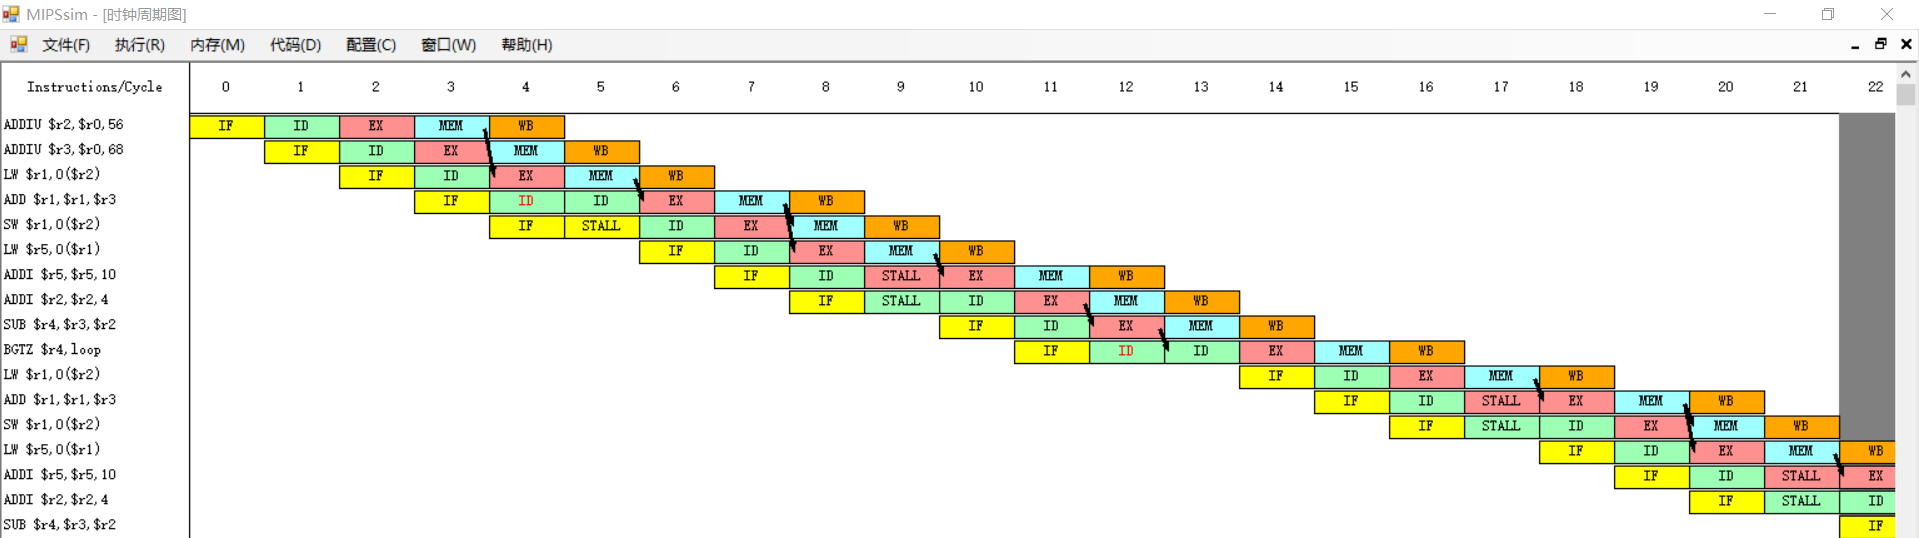
\includegraphics[width=1\textwidth]{fig/bypass.png}
                  \caption{时钟周期图}
                  \label{fig:bypass}
                \end{figure}

          \item 记录数据冲突引起的停顿周期数以及程序执行的总周期数。计算采用定向以后性能比原来提高多少。

                \textcolor{ans} {停顿周期:9}

                \textcolor{ans} {总周期:43}

                \textcolor{ans} {性能提升:65 / 43 = 1.51}

                \textcolor{ans} {占比:20.93023\%}

                \textcolor{ans}{运行报告:}
                \begin{lstlisting}
  汇总:
    执行周期总数:43
    ID段执行了29条指令

  硬件配置:
    内存容量:4096 B
    加法器个数:1		执行时间(周期数):6
    乘法器个数:1		执行时间(周期数)7		
    除法器个数:1		执行时间(周期数)10		
    定向机制:采用

  停顿(周期数):
    RAW停顿:9		占周期总数的百分比:20.93023%
    其中:
      load停顿:6		占所有RAW停顿的百分比:66.66666%
      浮点停顿:0		占所有RAW停顿的百分比:0%
    WAW停顿:0		占周期总数的百分比:0%
    结构停顿:0		占周期总数的百分比:0%
    控制停顿:3		占周期总数的百分比:6.976744%
    自陷停顿:1		占周期总数的百分比:2.325581%
    停顿周期总数:13	占周期总数的百分比:30.23256%

  分支指令:
    指令条数:3		占指令总数的百分比:10.34483%
    其中:
      分支成功:2		占分支指令数的百分比:66.66666%
      分支失败:1		占分支指令数的百分比:33.33333%

  load/store指令:
    指令条数:9		占指令总数的百分比:31.03448%
    其中:
      load:6		占load/store指令数的百分比:66.66666%
      store:3		占load/store指令数的百分比:33.33333%

  浮点指令:
    指令条数:0		占指令总数的百分比:0%
    其中:
      加法:0		占浮点指令数的百分比:0%
      乘法:0		占浮点指令数的百分比:0%
      除法:0		占浮点指令数的百分比:0%

  自陷指令:
    指令条数:1		占指令总数的百分比:3.448276%
\end{lstlisting}
        \end{itemize}
\end{enumerate}

\section{实验中的问题与心得}

本次实验大部分时间是在按部就班的运行别人的代码,实验中没有遇到任何问题。

至于心得,个人认为是测试程序很好地体现了旁路技术带来的性能优化。

\end{document}